% Figure from MATH 556 notes, section 10. Compile with the notes preamble.
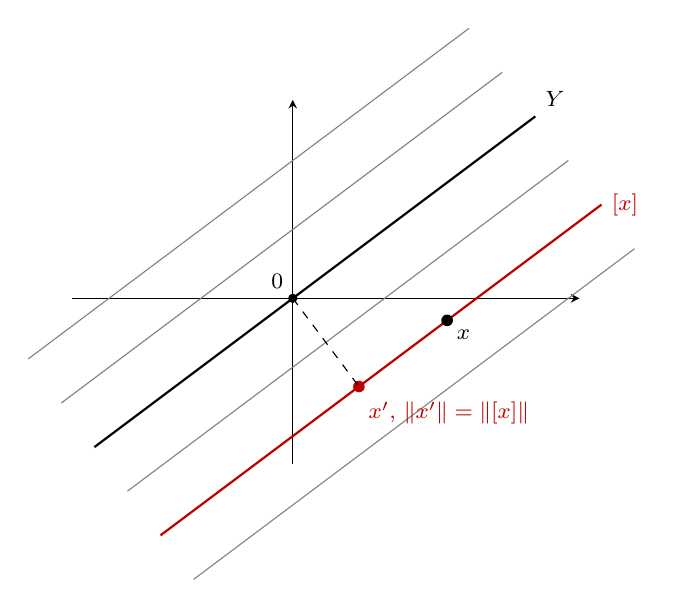
\begin{tikzpicture}[scale=1.4, >=stealth]
    \draw[->] (-2.0,0) -- (2.6,0) node[right] {};
    \draw[->] (0,-1.5) -- (0,1.8) node[above] {};
    % Y and parallel classes
    \draw[thick] (-1.8,-1.35) -- (2.2,1.65) node[above right, font=\footnotesize] {$Y$};
    \foreach \c in {-1.0,-0.5,0.5,1.5} {
        \draw[thin, gray] ({-1.8+\c*0.6},{-1.35-\c*0.8}) -- ({2.2+\c*0.6},{1.65-\c*0.8});
    }
    \draw[thick, red!75!black] ({-1.8+0.6},{-1.35-0.8}) -- ({2.2+0.6},{1.65-0.8}) node[right, font=\footnotesize] {$[x]$};
    % x on the red line
    \fill (1.4,-0.2) circle (1.5pt) node[below right, font=\footnotesize] {$x$};
    % closest point: foot of perpendicular from 0 onto red line (direction (4,3)/5, offset (0.6,-0.8))
    \fill[red!75!black] (0.6,-0.8) circle (1.5pt);
    \draw[dashed] (0,0) -- (0.6,-0.8);
    \node[below right, font=\footnotesize, red!75!black, yshift=-2pt] at (0.6,-0.8) {$x'$, $\|x'\| = \|[x]\|$};
    \fill (0,0) circle (1.2pt) node[above left, font=\footnotesize] {$0$};
\end{tikzpicture}
